\chapter{GPU-accelerated Mahalanobis-average Hierarchical Clustering Analysis}


% %
% \titlerunning{GPU-accelerated Mahalanobis Clustering}
% % If the paper title is too long for the running head, you can set
% % an abbreviated paper title here
% %
% \author{Adam Šmelko\inst{1}\orcidID{0000-0001-8334-2783} \and %
%  Miroslav Kratochvíl\inst{1,2}\orcidID{0000-0001-7356-4075} \and %
%  Martin Kruliš\inst{1}\orcidID{0000-0002-0985-8949} \and %
%  Tomáš Sieger\inst{3}\orcidID{0000-0003-4960-1934}}
% %
% \authorrunning{Šmelko et al.}
% % First names are abbreviated in the running head.
% % If there are more than two authors, 'et al.' is used.
% %
% \institute{Department of Software Engineering, Charles University, Prague\and Luxembourg Centre for Systems Biomedicine, University of Luxembourg, Esch-sur-Alzette\and Department of Cybernetics, Faculty of Electrical Engineering, Czech Technical University in Prague}
% %
% \maketitle              % typeset the header of the contribution
% %
% \begin{abstract}
% Hierarchical clustering is a common tool for simplification, exploration, and analysis of datasets in many areas of research.
% For data originating in flow cytometry, a specific variant of agglomerative clustering based Mahalanobis-average linkage has been shown to produce results better than the common linkages.
% However, the high complexity of computing the distance limits the applicability of the algorithm to datasets obtained from current equipment.
% We propose an optimized, GPU-accelerated open-source implementation of the Mahalanobis-average hierarchical clustering that improves the algorithm performance by over two orders of magnitude, thus allowing it to scale to the large datasets.
% We provide a detailed analysis of the optimizations and collected experimental results that are also portable to other hierarchical clustering algorithms; and demonstrate the use on realistic high-dimensional datasets.

% \keywords{clustering \and high-dimensional \and Mahalanobis distance \and parallel \and GPU \and CUDA.}
% \end{abstract}

% -----------------------------------------------------------------------------
\section{Introduction}
% -----------------------------------------------------------------------------

Clustering algorithms are used as common components of many computation pipelines in data analysis and knowledge mining, enabling simplification and classification of huge numbers of observations into separate groups of similar data.
Atop of that, a hierarchical clustering analysis (HCA) captures individual relations between clusters of data in a tree-like structure of dataset subsets (a \emph{dendrogram}), where each subtree layer corresponds to a finer level of detail.
The tree structure is suitable for many scenarios where the definition of clusters is unclear, such as in interactive analysis of noisy data where the assumptions of non-hierarchical algorithms (such as the requirement for apriori knowledge of cluster number of $k$-means) are not available.
Remarkably, the dendrogram output form of HCA provides an ad-hoc dataset ontology which has proven more intuitive for data inspection than the outputs of many other common clustering methods that yield unstructured results.

Here, we focus on hierarchical clustering applications on datasets that originate in flow cytometry, a data acquisition method that allows to quickly measure many biochemical properties of millions of single cells from living organisms.
Its widespread use has reached many diverse areas of science including immunology, clinical oncology, marine biology, and developmental biology.
The size of the obtained datasets is constantly growing, which naturally drives the demand for fast data processing and advanced analysis methods~\cite{lugli2010data}.
From the plethora of developed algorithms, clustering approaches allow easy separation of the measured single cell data into groups that usually correspond to the naturally occurring cell populations and types.
Hierarchical clustering improves the result by capturing and revealing more detailed relations between different types of cells.

A dataset from flow cytometry is usually represented as a point cloud in a multidimensional vector space, where each point represents a single measured cell and each dimension represents one measured `property', typically a presence of some selected surface proteins.
Recent hardware development has allowed simple, cheap acquisition of high-quality datasets of several million cells and several dozen of dimensions.

One of the issues in the analysis of this vector space is that the relations between individual dimensions are rather complex, and utilization of simple Euclidean metrics for describing data point similarity is rarely optimal.
Fišer et al.~\cite{fivser2012detection} have demonstrated the viability of specialized hierarchical clustering analysis method that uses Mahalanobis distance (MHCA) that captures cell clusters of ellipsoid shapes, which are common in cell populations (demonstrated in Figure~\ref{fig:mahaclust}).
Although this approach has proven to detect various elusive dataset phenomena, its scalability remained a concern.
In particular, the high computational cost of Mahalanobis distance makes the straightforward implementation on common hardware practically useful only for datasets of up to approximately $10^4$ cells.

\begin{figure}[t]
	\centering
	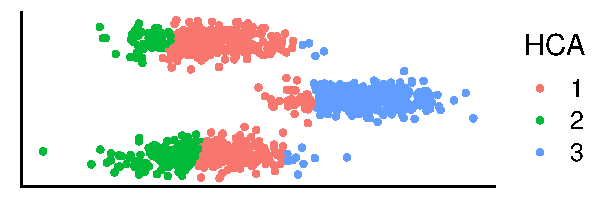
\includegraphics[width=2in]{Mahalanobis/img/hca.pdf}\quad%
	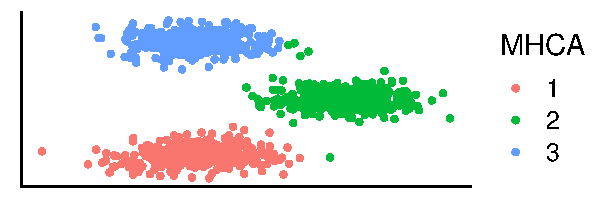
\includegraphics[width=2in]{Mahalanobis/img/mhca.pdf}
	\caption{Mahalanobis-based clustering (MHCA, right) captures the prolonged ellipsoid clusters better than commonly used hierarchical clustering (HCA, left)}
	\label{fig:mahaclust}
\end{figure}

\subsection{Contributions and Outline}

In the domain of clustering, algorithm performance has often been successfully improved by proper reimplementation for GPU hardware accelerators~\cite{krulivs2020detailed,gowanlock2017clustering,cuomo2019gpu}.
However, the computation of the MHCA is relatively irregular and rather complex, making the usual acceleration approaches ineffective.

As the main contribution of this paper, we describe our adaptation of MHCA for contemporary GPUs.
In particular, we describe a data structure that can be used to accelerate HCA algorithms on GPUs in general, and provide additional insight about efficiency of the specific parts of MHCA algorithm.
We subjected the implementation to comprehensive experimental evaluation and compared it with the existing implementation of MHCA to measure the achieved speedup.
Finally, we made the implementation available as open-source\footnote{\url{https://github.com/asmelko/gmhc}}, making it useful for both biological research and further experiments with parallelization of HCAs.

The mathematical and algorithmic overview of MHCA clustering is presented in Section~\ref{sec:mhca}, Section~\ref{sec:implementation} describes our proposed GPU implementation. We summarize the experimental evaluation in Section~\ref{sec:experiments}. Section~\ref{sec:relwork} puts the our research in proper context with prior work and Section~\ref{sec:conclusions} concludes the paper.


\section{Hierarchical Clustering with Mahalanobis Distance}\label{sec:mhca}
\label{sec:maha}

In this section, we review the necessary formalism and show the Mahalanobis average-linked hierarchical clustering algorithm.
The input dataset is a set of points in $d$-dimensional vector space, here assumed in $\mathbb{R}^d$, which is a common representation for cytometry data~\cite{shapiro2005practical}.
The algorithm produces a binary tree of \emph{clusters} where each resulting cluster is a subset of the input dataset of highly similar (`close' by some metric in the vector space) points.

Mahalanobis distance~\cite{mahalanobis1936generalized} is defined between a point $x$ and a non-singleton set of compact points $P$ as
\[ \delta_M(x,P) = \sqrt{(x-\bar{P})^T(\cov P)^{-1}(x-\bar{P})}, \]
where $\bar{P}$ is the centroid (mean) of the set $P$, and the entries of the covariance matrix are computed as
\[ (\cov P)_{ij} = \left(|P|-1\right)^{-1}\cdot \sum_{p \in P}{(p_i - \bar{P}_i)\cdot(p_j - \bar{P}_j)}. \]

One can intuitively view Mahalanobis distance as an Euclidean distance from the cluster centroid that also reflects the shape and the size of the cluster.
In particular, in a space that has been linearly transformed so that the covariance matrix of the cluster is a unit matrix, Euclidean and Mahalanobis distance coincide, as shown in Figure~\ref{fig:maha}.

\begin{figure}[t]
\centering
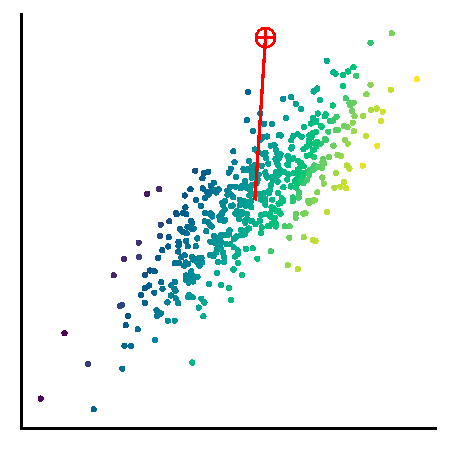
\includegraphics[width=1in]{Mahalanobis/img/maha1.pdf}\quad%
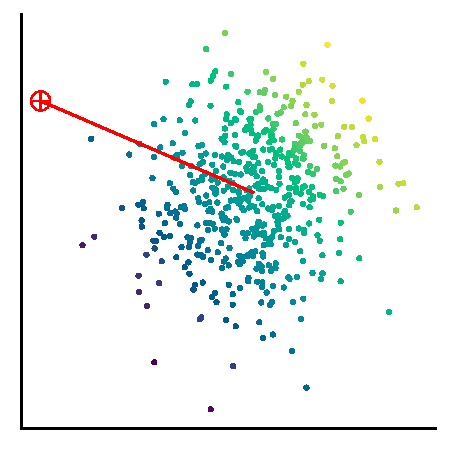
\includegraphics[width=1in]{Mahalanobis/img/maha2.pdf}
\caption{Mahalanobis distance (left) can be perceived as Euclidean distance (right) in a linearly transformed space where the cluster is perfectly `round'.
}
\label{fig:maha}
\end{figure}

The MHCA algorithm can be described in steps as follows:
\begin{enumerate}
	\item \emph{Initialization}: Construct an `active set' of numbered clusters $P_{1,2,\dots,n}$, each comprising one input element (data point) as $P_i=\{e_i\}$ for each $i \in \{1\ldots n\}$ where $\{e_1,\dots,e_n\}$ denotes the input dataset.
	\item \emph{Iteration}: Until the active set contains only a single item, repeat the following:

	\begin{enumerate}
		\item Compute pairwise dissimilarities of all clusters in $A$, select the pair $(P_r, P_s)$ with lowest dissimilarity. Output pair $(r,s)$.
		\item Update the active set by removing $P_r, P_s$ and adding $P_{n+i} = P_r\cup P_s$, where $i>0$ is an iteration number.
	\end{enumerate}

	\item \emph{Result}: the binary tree is specified by the trace of $n-1$ pairs $(r,s)$.
\end{enumerate}

Properties of the output depend mainly on the exact definition of the dissimilarity function used in step 2.a.
The common choices include the common `single' linkage (minimum pairwise distance between the 2 points in different clusters), `complete' linkage (maximum distance), `average' linkage (mean distance across clusters), `centroid' linkage (distance of cluster centroids), and others.
The used distance is usually a metric in the vector space, such as Euclidean.
The choice of the dissimilarity calculation methods is critical for obtaining results suitable for given analysis; the available methods have been therefore been subjected to much optimization~\cite{shirkhorshidi2015comparison}.

\subsection{Mahalanobis dissimilarity}

Fišer et al.~\cite{fivser2012detection} proposed the \emph{full Mahalanobis distance} as a dissimilarity function for HCA as an average of all Mahalanobis distances across clusters, as $\text{FMD}(P_i, P_j) = (|P_i|+|P_j|)^{-1} \left(\sum_k \delta_M((P_i)_k, P_j) + \sum_k\delta_M((P_j)_k, P_i)\right)$.
While this construction is intuitively correct and allows the clustering to precisely capture various dataset phenomena that are common in cytometry, the definition opens many inefficiencies and border cases that need to be resolved:

\begin{itemize}
	\item Mahalanobis distance may be undefined for small clusters because the covariance matrix is singular or nearly-singular. This can be resolved by a complete or partial fallback to robust distance measures, as detailed in Section~\ref{sec:maho-singular}.
	\item Because the Mahalanobis distance of a fixed point to a cluster \emph{decreases} when the cluster size increases (e.g., as a result of being merged with another cluster), the minimal dissimilarity selected in the step 3 of the algorithm may sometimes be smaller than the previously selected one.
  A correction is thus needed to keep the dissimilarity sequence properly monotonic, giving uncluttered, interpretable dendrogram display~\cite{everitt2002cambridge}.
	\item The amount of required computation is significantly higher than with the other linkages (dissimilarity functions), requiring additional operations for computing the inverted covariance matrix and covariance-scaled Euclidean distances.
  We mitigate this problem by massive parallelization with GPU accelerators, as detailed in Section~\ref{sec:implementation}.
\end{itemize}

The computation of the `full' average Manalanobis distance is unavoidably demanding, requiring many matrix-vector multiplications to compute distances between all points of one cluster and the opposite cluster.
Following the variations of Euclidean dissimilarity measures for HCA, a \emph{centroid-based Mahalanobis distance} may be specified to use only the average of the distance to the centroids of the other cluster, as $\text{CMD}(P_i, P_j) = \frac{1}{2} \left(\delta_M(\bar{P_i}, P_j) + \delta_M(\bar{P_j}, P_i)\right)$.
The result may be viewed as a fast approximate substitute for the full variant because the simplification removes a significant portion of the computational overhead and still produces sound results in many cases.
The difference between CMD and FMD is highly pronounced only when the centroids of the clusters are near, but their respective covariances differ, as visualized in Figure~\ref{fig:maha_var}.
Fortunately, such situations are quite rare in clustering of realistic datasets.

\begin{figure}[t]
  \centering
	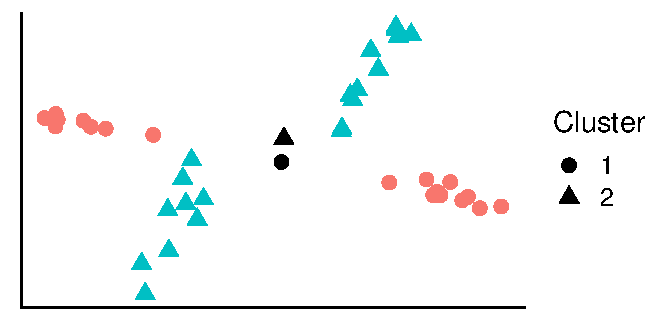
\includegraphics[width=2.2in]{Mahalanobis/img/dists.pdf}
	\caption{An example of two clusters for which the CMD fails to satisfactorily approximate the FMD (centroids are plotted in black).}
	\label{fig:maha_var}
\end{figure}

\subsection{Singularity of cluster covariance matrix}\label{sec:maho-singular}

In early iterations of MHCA, the clusters consist of only a few points.
Covariance matrix of a small cluster is likely singular, which means it is impossible to compute its inverse required by the Mahalanobis distance measure.
Furthermore, even for more points the covariance matrix may be nearly singular, and using its ill-conditioned inverse will yield inaccurate results and numeric floating-point anomalies (such as negative distances or infinities).

To solve this problem, Fišer et al.~\cite{fivser2012detection} proposed the following approach:
If the number of elements in a cluster relative to whole dataset size is lower than a threshold, the covariance matrix of such cluster is transformed so it can be inverted, and handled in a numerically safe manner.
We will denote the used threshold as the \emph{Mahalanobis threshold}, and categorize the clusters as \emph{sub-threshold} and \emph{super-threshold cluster}, depending on their size being below and above the Mahalanobis threshold respectively.

We later explore the following \emph{subthreshold handling methods} for managing the problematic covariance matrix values:
\begin{itemize}
	\item \textsc{Mahal} smoothly pushes the vectors of the covariance matrices of the sub-threshold clusters towards a unit sphere, so that the space around the clusters is not excessively distorted (or projected).
	\item \textsc{EuclidMahal} enforces unit (spherical) covariance vectors of the sub-thres\-hold clusters (thus enforcing Euclidean distances).
    Despite the simplicity and effectiveness, the hard thresholding may lead to a non-intuitive behavior; for example, the merging of a pair of large elliptical clusters that are just above the threshold may be prioritized over a pair of more similar but sub-threshold clusters.
	\item \textsc{Euclid} enforces unit covariances of all clusters \emph{only until the last sub-threshold cluster is merged}.
    This option usually leads to a viable formation of compact clusters, but completely ignores the possible intrinsic structure of several super-threshold clusters.
\end{itemize}

\subsection{Complexity and parallelization opportunities of MHCA}

A straightforward serial implementation of MHCA (such as the implementation in \texttt{mhca} R package\footnote{\url{https://rdrr.io/github/tsieger/mhca}}) works with iterative updates of the dissimilarity matrix.
Let us examine in detail the time complexity of the individual algorithm steps on a dataset that contains $n$ points of $d$ dimensions:

First, the algorithm constructs a dissimilarity matrix in $\mathcal{O}(d\cdot n^2)$, and identifies the most similar cluster pair in $\mathcal{O}(n^2)$. Then a total of $n-1$ iterations is performed as such:
\begin{itemize}
  \item a covariance matrix of the merged cluster is computed ($\mathcal{O}(d^2\cdot n)$) and inverted ($\mathcal{O}(d^3)$),
  \item the dissimilarity matrix is updated ($\mathcal{O}(d^2\cdot n)$), and
  \item the new most similar cluster pair is identified ($\mathcal{O}(n^2)$).
\end{itemize}

The total complexity is thus $\mathcal{O}(d\cdot n^2 + (n-1) \cdot (d^2\cdot n + d^3 + n^2))$.
Assuming $d\ll n$, the asymptotic complexity can be simplified to $\mathcal{O}(n^3)$.
Since we cache the unchanged dissimilarity matrix entries, the memory complexity is $\mathcal{O}(n^2)$.

In an idealized parallel execution environment (PRAM model with concurrent reads and infinite parallelism), we could improve the algorithm to perform faster as follows:
All cluster dissimilarity computations (including the later dissimilarity matrix update) can be performed in parallel in $\mathcal{O}{(d^3\cdot \log n)}$, using parallel reduction algorithm for computing the covariance sums.
The most similar cluster pair can be selected using a parallel reduction over the dissimilarity matrix in $\mathcal{O}(\log^2 n)$.
The total required time would thus be reduced to $\mathcal{O}(d^3 n\log^2 n)$ (again assuming $d\ll n$), using $\mathcal{O}(n^2)$ memory.

While this suggests two main ways of performance improvement for the massively parallel GPU implementation, the specifics of the current GPUs pose problems for such naive parallelization approach:
\begin{itemize}
	\item Parallelization of any single covariance matrix computation will improve performance only if the covariance matrix is sufficiently large, otherwise the performance may be reduced by scheduling overhead and limited parallelism.
	\item Scanning of the large dissimilarity matrix is parallelizable, but is hindered by relatively small amount of available GPU memory and insufficient memory throughput.
\end{itemize}

In the following section, we address these problems with optimizations that make the computation viable on the modern accelerators.
In particular, we show that the computation of a covariance matrix can be divided into many independent parts, thus exposing sufficient parallelization opportunities, and we demonstrate a technique for efficient caching of intermediate contents of the dissimilarity matrix to reduce the memory footprint and throughput requirements of the algorithm.

% -----------------------------------------------------------------------------
\section{GPU Implementation}\label{sec:implementation}
% -----------------------------------------------------------------------------

Memory handling optimizations form the essential part of our GPU implementation of MHCA, here called \emph{GMHC} for brevity.
Most importantly, we address the tremendous memory requirement of storing the dissimilarity matrix ($\mathcal{O}(n^2)$) for large $n$.
We replace this matrix with a special \emph{nearest-neighbor array}, which provides similar caching benefits, but requires only $\mathcal{O}(n)$ memory.
This saving in memory volume is redeemed by a slightly higher computational complexity; however, the measured improvement in scalability warrants this trade-off.

\begin{defn}[Nearest neighbor array]
	For clusters $P_1,\dots,P_n$ and a symmetric dissimilarity function $d$, the \emph{nearest neighbor array} $N$ contains $n-1$ elements defined as
	\[N_i = \argmin_{j>i} d(P_i,P_j).\]
	\label{def:nna}
\end{defn}

%(Symmetricity of $d$ is required to reduce the scope of $\argmin$ from original $j\neq i$.)

Maintaining a nearest neighbor array in the HCA computation allows us to reduce the amount of distance computations performed after each update.
In particular, when a cluster pair $(P_i,P_j)$ is merged into new cluster $P_m$, only elements with values $i$ and $j$ have to be recomputed, along with the new value for $N_m$

This is enabled by the symmetry of $d$, which allowed us to ensure that the contents of the nearest neighbor arrays at some index \emph{only depend on clusters with higher indices}.
If we set the new index $m$ to be smaller than all existing indices in the array (i.e., $m=1$, shifting the rest of the array), the newly appearing cluster can not invalidate the cached indices for the original array, and only the entries that refer to the disappearing clusters $i,j$ need to be recomputed.
In consequence, if an already present cluster $P_k$ was to form the most similar pair with the new cluster $P_m$, this information would be present the $\argmin_{k>m}$ computation, and stored in $N_m$ instead of $N_k$.

In an optimistic scenario, the above optimization can be used to limit the number of elements that need to be updated in each iteration by a constant number, which leads to a major increase in overall performance.
This constant limit is supported by empirical observations on realistic datasets with around 1 million of objects, where the number of triggered updates was rarely over $50$.
Further, we reduce the need for recomputation by caching several `nearest' neighbors for each entry of $N$:

\begin{defn}[Neighbor buffer]
A sorted list of $L$ nearest neighbor indices (respectively to the $\argmin_{j>i}$ in definition~\ref{def:nna}) stored for each item in $N$ is called a \emph{neighbor buffer}.
\end{defn}

To ensure the efficiency of the process, we split the update of neighbor buffers to two parts:
First, when $(P_i,P_j)$ is merged into $P_m$, all buffers are filtered and values $i$ and $j$ are removed (i.e, replaced with dummy values).
On recomputation, all empty buffers (including newly formed $N_m$) are filled with indices of nearest $L$ neighbors, while the partially filled buffers are left intact.
This allows us to reuse the intermediate results of the computation of an $N$ array entry for as much as $L$ recomputations that involve the cluster.

The complexity of updating the nearest neighbor array element $i$ for the neighbor buffer of size $L$ on $m$ clusters, using a pair dissimilarity computation of complexity $\mathcal{O}(\delta)$, is $\mathcal{O}((m-i)\cdot (\delta+L))$.
The reduced amount of index updates thus trades off for index update complexity, depending on $L$.
The optimal choice of $L$ is discussed later in Section~\ref{sec:exp}.

\subsection{Algorithm overview}

The hierarchical clustering of $n$ initial clusters is a series of $n-1$ iterations, such that in each iteration two clusters are merged into one. Before the first iteration, the nearest neighbor array $N$ must be initialized.
Each subsequent iteration comprises the following compact steps:
\begin{enumerate}
	\item Scan the neighbor array and fetch the most similar cluster pair
	\item Create a new cluster by merging the cluster pair
	      \subitem Compute its corresponding centroid and covariance matrix
	      \subitem Transform and invert the covariance matrix
	\item Update the neighbor array (only required if $n\geq 3$)
\end{enumerate}

\begin{figure}[t]
\centering
	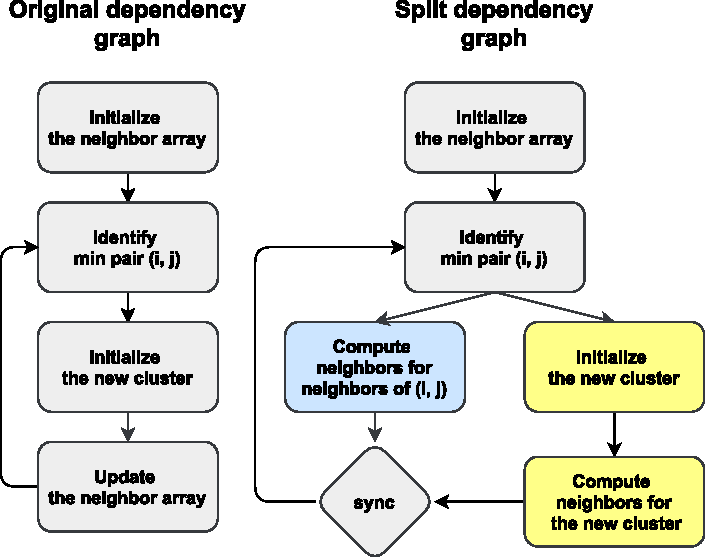
\includegraphics[width=8cm]{Mahalanobis/img/dependency-graph}
	\caption{The original graph of dependencies and the proposed split dependency graph, where blue and yellow boxes can be executed concurrently}
	\label{fig:dep-graph}
\end{figure}

The individual parts of the algorithm may be scheduled and executed dynamically, ordered only the data dependencies as displayed in Figure~\ref{fig:dep-graph}.
Mainly, this allows us to split the update of the neighbor array into update of the neighbors of old clusters ($i$, $j$) and the update of the newly created cluster.
Naturally, the individual steps are internally implemented as data-parallel operations as well.

In GMHC, we control the iteration loop from the host code, while the work of each update step is implemented within a CUDA kernel.
Our code employs CUDA streams~\cite{cuda} to efficiently implement the execution overlaps, creating some high-level task parallelism in the process.
In the rest of this section, we detail the implementations of the individual CUDA kernels.


\subsection{Cluster merging and covariance computation}

Covariance matrix $\cov P$ of cluster $P$ (and its inversion) is computed only when a cluster is formed; in our case when two clusters are merged.
In GMHC, we iterate over all data points $x \in P$ and each item $(\cov P)_{ij}$ is computed as a sum of centered products of $x_i$ and $x_j$ (following the definition from Section~\ref{sec:maha}).
As the most pressing issue, the performance of this process depends on fast finding of data points $x$ that belong to the cluster in the array of all data points.

A possible straightforward solution, storing an array of assigned points for each data cluster so that the assigned points can be accessed in a fast and compact way, would require dynamic memory allocation or manual apriori over-allocation, and many data moving operations.
We settled for a more compact solution with an assignment array that stores a cluster indices for each data point.
Although that does not require data copying, both the cluster merge and the retrieval of one cluster points will take $\mathcal{O}(n)$ time.
Fortunately, the two operations can be performed by a single parallel scan of the assignment array in this case.

\subsubsection{Covariance kernel implementation.}

The covariance kernel takes advantage of the symmetry of a covariance matrix and computes only its upper triangle.
Additionally, extra parallelism can be obtained by slicing the computation of the covariance matrix from Section~\ref{sec:maha} over individual data point contributions $\mathbf{S}^x$, as
$\cov P = (|P|-1)^{-1}\sum_{x\in P}\mathbf{S}^x$, where
$\mathbf{S}^x_{ij}=(x_i-\mathbf{\bar{x}}_i)\cdot(x_j-\mathbf{\bar{x}}_j)$.

The kernel is implemented as a loop over all data points.
A whole CUDA warp is assigned one data point and computes the intermediate $\mathbf{S}^x$.
These are then added together in a two-step reduction --- all intermediate states within a CUDA block are reduced using shared memory, which is then followed by a global reduction performed by a separate kernel launch that outputs the totals in a single covariance matrix.

Notably, the covariance matrices of single-point clusters are not computed; rather, they are assigned a default unit matrix.

\subsection{Inverse covariance storage optimization}
\label{subsec:icov}

The Mahalanobis distance requires inversion of the covariance matrix, which needs to be computed from the results of the previous step.
We use \texttt{cuSolver} library\footnote{\url{https://docs.nvidia.com/cuda/cusolver/index.html}} for implementing the matrix inversion, namely the routines \texttt{potrf} and \texttt{potri}.

The inverted matrix is subsequently transformed to better suit the Mahalanobis distance formula, and to eliminate redundant computations later in the process. In particular, we rewrite the Mahalanobis formula for inverse covariance matrix $M$ as a quadratic form
\[x^T M x =
  \sum_{i=1}^{d}\sum_{j=1}^{d}m_{ij}x_ix_j = \sum_{i=1}^{d}m_{ii}x_i^2 + \sum_{i=1}^{d}\sum_{j>i}^{d}2m_{ij}x_ix_j,\]
allowing us to store only the upper-triangular part of the matrix, pre-multiplied by $2$.

\subsection{Maintenance of nearest neighbor array}

GMHC implements 2 similar processes for the neighbor array initialization and update, differing mainly in the granularity of the task size.
We thus only focus on the update implementation.

First, specific simplified version of kernel for computing the distances is used for cases when the covariance matrix is unit, falling back to efficient implementation of Euclidean distance.
The decision which kernel to execute is done in the host code, depending solely on the selected subthreshold handling method (explained in Section~\ref{sec:maho-singular}) and the size of the two involved clusters.
The decision is formalized in Table~\ref{tab:neigh-select}.

\begin{table}[b]
	\centering
	%\setlength{\tabcolsep}{10pt}
	\begin{tabular}{@{}llll@{}}
		\toprule
		Subthreshold handling method~~ & sub/sub~~ & sub/super~~ & super/super \\
		\midrule
		\textsc{Euclid}      & \texttt{euclid} & \texttt{euclid} & \texttt{maha}  \\
		\textsc{EuclidMahal} & \texttt{euclid} & \texttt{maha}   & \texttt{maha}  \\
		\textsc{Mahal}       & \texttt{maha}   & \texttt{maha}   & \texttt{maha}  \\
		\bottomrule
	\end{tabular}
  \smallskip
	\caption{The host-side selection of the neighbor-distance kernel}
	\label{tab:neigh-select}
\end{table}


\subsubsection{The neighbor array update kernel.}

The update operation of nearest neighbor buffer array entry $N_i$ is defined as finding $L$ nearest clusters with index greater than $i$, and storing their ordered indices into $N_i$ neighbor buffer.
We split this operation in two parts, each handled by a separate kernel:
\begin{enumerate}
	\item Compute distances between all relevant cluster pairs concurrently.
	\item Reduce the results into a single nearest neighbor buffer entry.
\end{enumerate}

The execution of the first step differs between the Euclidean and the Mahalanobis neighbor computation.
While the former parallelizes trivially with one thread computing one distance value, the complex computation of Mahalanobis distance executes faster if the whole warp cooperates in one distance computation.

The precise operation needed to compute the Mahalanobis distance is a vector-matrix-vector multiplication.
To evaluate the formula from Section~\ref{subsec:icov}, we utilize the fuse-multiply-add intrinsic instructions to accumulate the results of the assigned work into their privatized buffers, which are subsequently reduced using fast warp-shuffle instructions.

In the second step, which selects the nearest $L$ indices, is the same for both distance measures.
We use a three-level implementation:
At the first level, the threads accumulate local minima of small array slices into their registers.
At the second level, each thread block utilizes the shared memory to efficiently exchange data and compute block-wise minima.
The third level collects the resulting minima and performs the same final reduction on a single thread block (thus efficiently utilizing intra-block synchronization).
The second and the third level could be fused together if the atomic instructions were used to synchronize data updates explicitly; however, we observed the improvement was negligible and preferred to reduce the design complexity instead.

This whole neighbor buffer `refill' operation is performed concurrently for every index in the nearest neighbor array that needs to be updated.
Our implementation executes a separate CUDA grid for each update, which reduces implementation complexity but still allows the grids to run concurrently and utilize the entire GPU.


% -----------------------------------------------------------------------------
\section{Experimental Results}\label{sec:experiments}
% -----------------------------------------------------------------------------

We have subjected our implementation of GMHC to extensive experimental evaluation, measuring the effect of main design choices in the algorithm.
In this section, we present the most important results and we put them in proper context, particularly with respect to parameter selection and scaling.

\subsection{Benchmarking methodology and datasets}

The experiments were performed on two systems --- a high-end server equipped with NVIDIA Tesla V100 SXM2 (32 GB) and a mainstream PC with NVIDIA GeForce GTX 980 (4 GB).
Both systems used Linux CentOS 8 with CUDA Toolkit (11.2).

We used the original MHCA clustering implementation by Fišer et al.~\cite{fivser2012detection} as a baseline, which is, to our best knowledge, the only other publicly available MHCA implementation.
The baseline algorithm is written in C as strictly sequential without explicit utilization of SIMD instructions; but it properly utilizes the highly-optimized \texttt{Blas} library for most heavy computation.
It was benchmarked on a high-end server with Intel Xeon Gold 5218 CPU, clocked at $2.3$~GHz (with 64 logical cores) and $384$~GB RAM (the same as the high-end server used for benchmarking GMHC).
We stress that the comparison between CPU and GPU implementation is not entirely objective, and the test results should be perceived more as a measure of overall data capacity improvement than of the implementation quality.
We did not test MHCA on the mainstream PC platform, because of the enormous $\mathcal{O}(n^2)$ memory requirements totaled to hundreds of gigabytes in our benchmarks.

As testing data, we used several high-dimensional datasets originating in mass cytometry~\cite{weber2016comparison}, namely the \texttt{Nilsson\_rare} (44K data points, 14 dimensions), \texttt{Levine\_32dim} (265K data points, 32 dimensions) and \texttt{Mosmann\_rare} (400k data points, 15 dimensions).
For brevity, we report only a subset of the measured results, but these should generalize well to other data.
In particular, we did not observe any significant data-dependent performance differences.

In all experiments, we measured the wall time of the total algorithm execution.
The experiments were performed multiple times to prevent random deviations in measurement; we display mean values of the measurements.
Because the experimental evaluations on both mentioned GPUs behaved consistently with no surprising differences on any particular hardware, we present mainly the results from Tesla V100 SXM2 GPU unless stated otherwise.

\subsection{Experiment results}\label{sec:exp}

First, we evaluated the scalability of the GMHC implementation depending on the size of the dataset.
The inputs of different sizes were achieved by randomly sub-sampling the Mosmann dataset.
Figure~\ref{fig:perf_methods} shows the wall time for each subthreshold method, revealing that the performance scales sub-quadratically with data size.
Notably, the optimized implementations of \textsc{Euclid} and \textsc{EuclidMahal} scale about $10\times$ better than full \textsc{Mahal} for this dimensionality.

\begin{figure}[t]
	\centering
	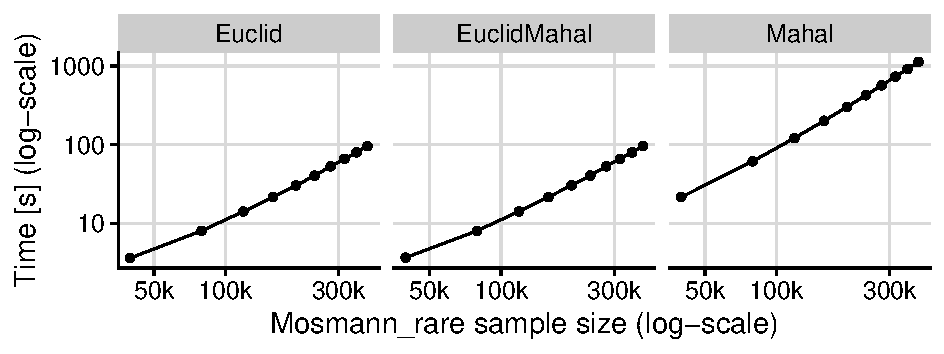
\includegraphics[width=8cm]{Mahalanobis/img/methods.pdf}
	\caption{Comparison of the subthreshold distance computation method performance.}
	\label{fig:perf_methods}
\end{figure}

The tradeoff between Euclidean and Mahalanobis computation in the first two methods can be further controlled by setting the threshold value $t$, controlling whether a cluster is considered small or large, and in turn, deciding the dissimilarity metric to use.
Figure~\ref{fig:perf_thresh} summarizes the performance gains for various setting of this threshold.

\begin{figure}[t]
	\centering
	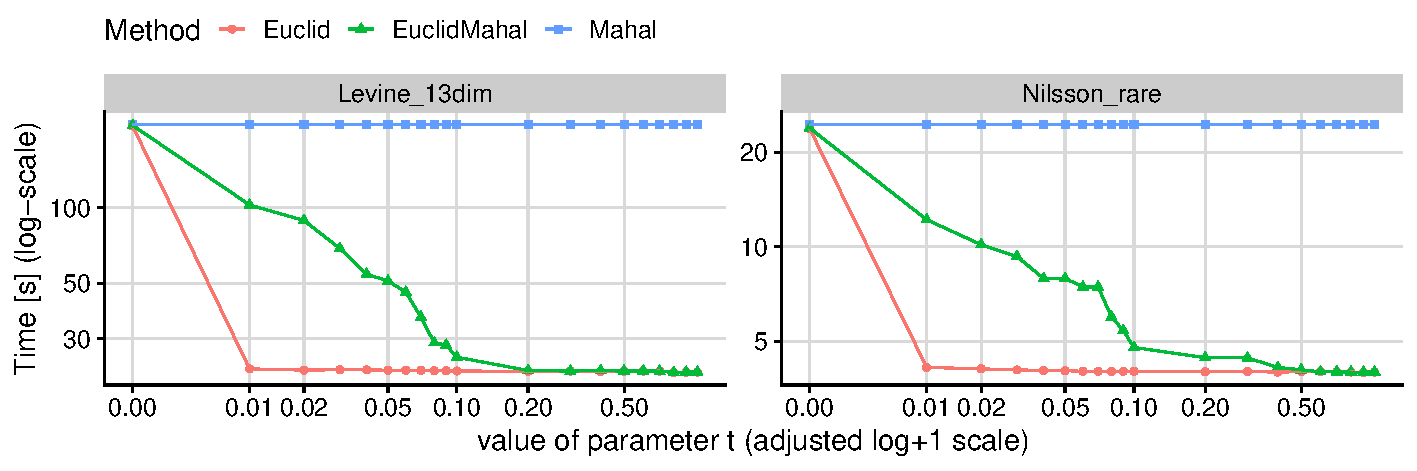
\includegraphics[width=12cm]{Mahalanobis/img/thresh.pdf}
	\caption{Clustering time of subthreshold methods with varying Mahalanobis threshold value on two different datasets.}
	\label{fig:perf_thresh}
\end{figure}

In the figure, $t=0$ forces all methods perform dissimilarity measurements using the Mahalanobis distance. When we increase $t$ only very slightly to $0.01$, the \textsc{Euclid} method time decreases dramatically and stays almost the same in the remainder of $t$ range. This is often caused by small sub-threshold clusters that are propagated to the very end of the clustering, which postpones the switch to the Mahalanobis distance. On the other hand, the \textsc{EuclidMahal} method shifts its wall time smoothly towards the \textsc{Euclid} method as $t$ increases, which is a consequence of the first super-threshold cluster appearing later in the process.

To determine the optimal value of the nearest neighbor buffer size, we benchmarked the clustering of datasets with a range of parameters $L$ (Figure~\ref{fig:perf_nei}).

\begin{figure}[t]
	\centering
	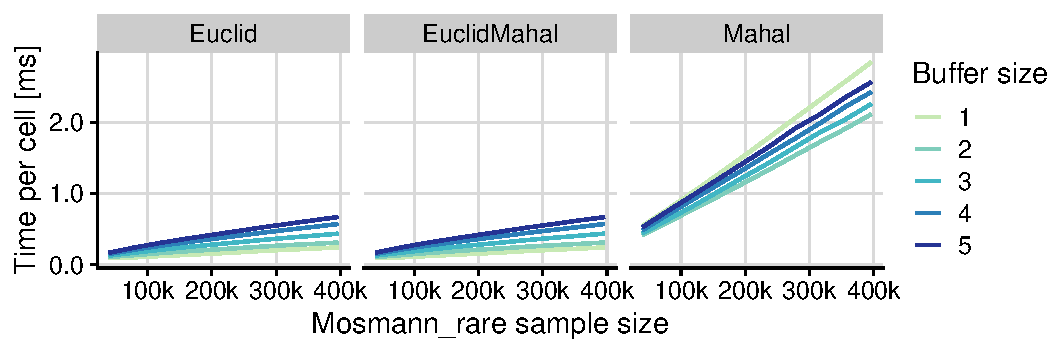
\includegraphics[width=9cm]{Mahalanobis/img/neighbors.pdf}
	\caption{Comparison of neighbor buffer sizes for subthreshold methods ($t=0.5$)}
	\label{fig:perf_nei}
\end{figure}

Curiously, the observed results show that while $L=1$ is optimal for \textsc{Euclid} and \textsc{EuclidMahal}, it performs worst for \textsc{Mahal} method. This is a consequence of the used distance function in dissimilarity measurements --- for the \textsc{Euclid} and \textsc{EuclidMahal} method, where the Euclidean distance function dominates, the time difference for performing smaller number of neighbor updates did not balance the increased time complexity of a single update. The \textsc{Mahal} method works optimally with $L=2$; as the $L$ increases further, the performance starts to decrease again. 

Similarly, the optimal value of $L$ increases for higher-dimensional datasets, which we tested on Levine\_32dim data (detailed results not shown). In particular, for Mahalanobis distance, we measured the same optimal value $L=2$ with much greater performance gain (over $30\%$) against $L=1$ than on the Mosmann dataset. We expect that the optimal value of $L$ will continue to increase with the dimensionality of the dataset in case of the \textsc{Mahal} method. On the other hand, the Euclidean-based methods kept their optimum at $L=1$.

\begin{figure}[t]
	\centering
	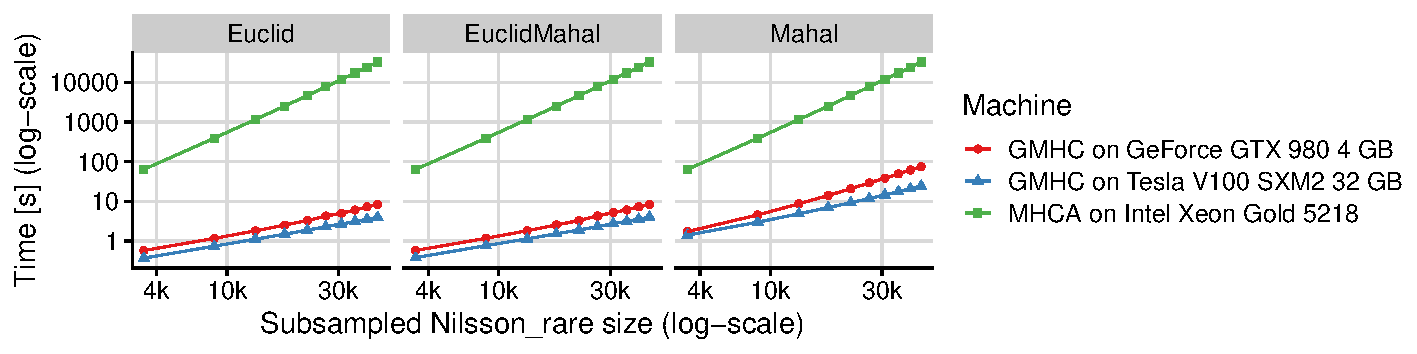
\includegraphics[width=12cm]{Mahalanobis/img/comparison.pdf}
	\caption{GMHC and MHCA comparison on Nilsson dataset with default $t=0.5$.}
	\label{fig:perf_comp}
\end{figure}

Finally, we compared the performance of GPU implementation of MHCA to the CPU baseline, to estimate the outcome for practical data analysis scalability.
Figure~\ref{fig:perf_comp}) indicates an overall performance increase by up to $1400\times$ in case of the \textsc{Mahal} method and by up to $8000\times$ in case of mixed-Euclidean methods.
When comparing performance on the older `gaming' GTX 980 GPU, the speedups were around $400\times$ and $4000\times$, respectively.
In summary, modern GPUs have been able to accelerate the MHCA task by more than three orders of magnitude, which is consistent with the effects of parallelization applied to many other clustering algorithms.


% -----------------------------------------------------------------------------
\section{Related Work}\label{sec:relwork}
% -----------------------------------------------------------------------------

The original version of MHCA clustering for flow cytometry by Fišer~et~al.~\cite{fivser2012detection} used a MATLAB implementation to analyze datasets of around $10^4$ multi-dimensional data points.
Due to the limited scalability and interoperability with modern data analysis environments, a C version of the algorithm has been implemented within R package \texttt{mhca} and enhanced with the possibility of assuming apriori clusters for approximation, to reduce the unfavorable $\mathcal{O}(n^3)$ time complexity for large datasets.
That allowed the authors to process datasets of around $10^6$ data points within an interactive environments~\cite{kratochvil2020shinysom}.

Despite of the performance advancement, the approximation in the method did not retain the sensitivity required to detect various small clusters of interest (i.e., small cell populations), such as the `minimum residual disease' cells crucial for diagnosis of acute myeloid leukemia~\cite{fivser2012detection}.
Similar approximations are used in many other clustering methods to gain performance at the cost of precision justifiable in a specific domain; including the 2-level meta-clustering approach of FlowSOM~\cite{gassen2015flowsom}, and advanced approximate neighborhood graph structure of FastPG~\cite{fastpg}.

Acceleration of HCAs on GPUs has been explored by several authors:
Chang et al.~\cite{chang2009hierarchical} discuss hierarchical clustering of gene mRNA levels assayable by DNA microarray technology.
Their GPU code computes matrix of pairwise distances between genes using Pearson correlation coefficient as one of the present metrics, and utilized a special property of data to effectively perform single-linkage over the present matrix.
Zhang et al.~\cite{zhang2006hierarchical} used similar clustering methodology, but employed GPU texture elements for the data representation of gene expression profile HCA.
Both acceleration methods resulted in performance increase between $5\times$ to $30\times$ on datasets of $10^4$ data points.


% -----------------------------------------------------------------------------
\section{Conclusions}\label{sec:conclusions}
% -----------------------------------------------------------------------------

We have presented an implementation approach for Mahalanobis-average linkage hierarchical clustering algorithm, which utilizes modern parallel GPU accelerators to increase its performance.
In the benchmarks, our GPU implementation GMHC has achieved over $10^3\times$ speedup on practical datasets over the current CPU implementations, which enabled scaling of the MHCA algorithm to large datasets produced by current data acquisition methods.

Together with the open-source implementation, we have provided a new high-performance building block for dataset analyses which should support the growing demand for fast data analysis methods not only in cytometry, but also in other areas of data analysis dealing with irregularly shaped Gaussian clusters.

The implementation structure detailed in the paper has allowed us to streamline the utilization of parallel hardware for accelerating general hierarchical clustering algorithms.
We expect that the proposed data structures will be ported to support acceleration of dissimilarity measures in other hierarchical clustering methods, providing a solid building block for future acceleration of data mining and knowledge discovery.


% \subsection*{Acknowledgements}

% This work was supported by Czech Science Foundation (GAČR) project 19-22071Y,
% by ELIXIR CZ LM2018131 (MEYS),
% by Charles University grant SVV-260451,
% and by Czech Health Research Council (AZV) [NV18-08-00385].

